\chapter{Introduction}





4-hydroxy-methyl-pyridine and 4-methoxy-pyridine are compounds which, despite being easy to handle, see little use in synthesis of coordination compounds. This is evident in the lack of published crystal structures containing them - currently 34 contain the first and only 23 the latter one. \cite{ccdc} Most of these complexes employ transition metals like platinum, nickel or silver as central atom. Also only a few of them have pseudohalides as ligands.\\


\begin{figure}[htpb!]
\centering
\subfigure[]{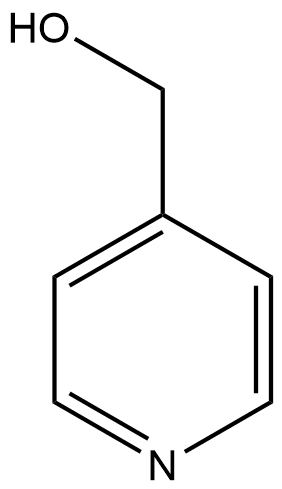
\includegraphics[scale=0.30]{figures/4HOMP.png}}
\quad
\subfigure[]{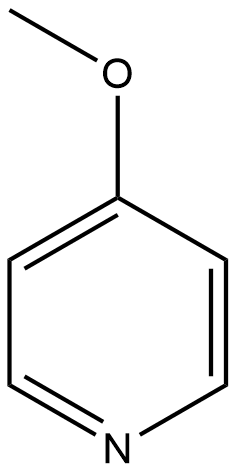
\includegraphics[scale=0.30]{figures/4-MOP.png}}
\caption{4-hydroxy-methyl-pyridine (a) and 4-methoxy-pyridine (b)}
\label{fig:4mophomp}
\end{figure}

The aim of this master thesis was the synthesis, spectral and structural characterization of new transition metal complexes using aforementioned pyridines with pseudohalides and transition metals.
Pseudohalides were chosen  as anionic ligands due to their similar properties to halides.  The central metal can bind to the end or middle atoms of these polyatomic ligands, making various combinations possible.\\

Mixing ligands and metal salts with varying ratios results in complexes with different coordination numbers (CN). Coordination numbers describe the number of donor atoms contained by ligands which are surrounding the central atom. 2, 4, 5 and 6 are common coordination numbers.\\

For the coordination number 2 only linear arrangements are  known and these complexes are often formed with the single positively charged ions \ce{Ag^+}, \ce{Cu^+} and \ce{Au^+}. \cite{riedel} \\

Tetrahedral and square-planar arrangements are possible for coordination number 4. Tetrahedral complexes are more common and are formed in all kinds of d-configurations whereas d$^8$-configuration (or 16-electron-complexes) prefer the square planar arrangement, i.e. \ce{Pt^{2+}} or \ce{Pd^{2+}}. \cite{riedel}   \\

Square-pyramidal and trigonal-bipyramidal structures are forms of the seldom appearing coordination number 5. They can be transformed into each other via Berry rotation \cite{berry} and are in equilibirium at a certain temperature.

CN 6 forms are octahedron (common), trigonal antiprism or trigonal prism (rare). The metal ions \ce{Cr^{3+}}, \ce{Co^{3+}} and  \ce{Pt^{3+}} favor the octahedral arrangement.\cite{riedel} \\

 
 The coordination numbers with their frequent arrangements are listed in figure \ref{fig:kz}.

\begin{figure}
\centering
\subfigure[CN2: linear]{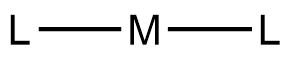
\includegraphics[width=0.30\linewidth]{figures/linear.png}}
\subfigure[CN4: square-planar]{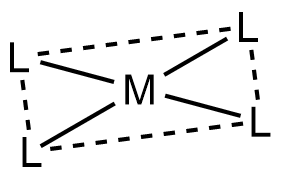
\includegraphics[width=0.30\linewidth]{figures/square-planar.png}}
\subfigure[CN4: tetrahedral]{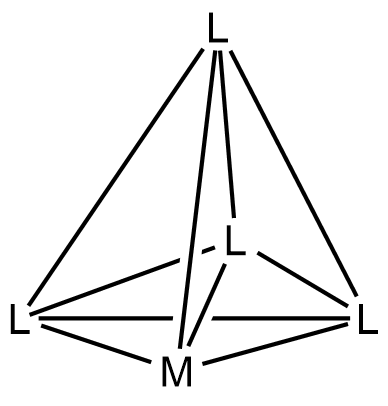
\includegraphics[width=0.30\linewidth]{figures/tetrahedral.png}}

\subfigure[CN5: square-pyramidal]{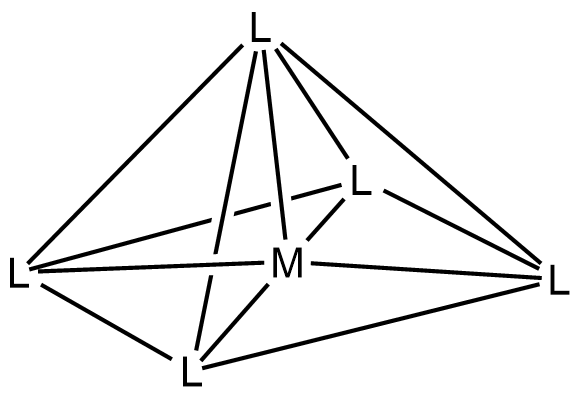
\includegraphics[width=0.30\linewidth]{figures/square-pyramidal.png}}
\subfigure[CN5: trigonal-bipyramidal]{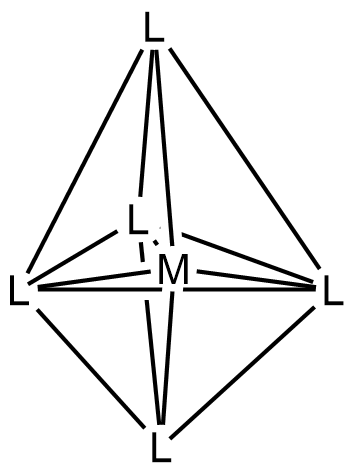
\includegraphics[width=0.30\linewidth]{figures/trigonal-bipyramidal.png}}
\subfigure[CN6: octahedral]{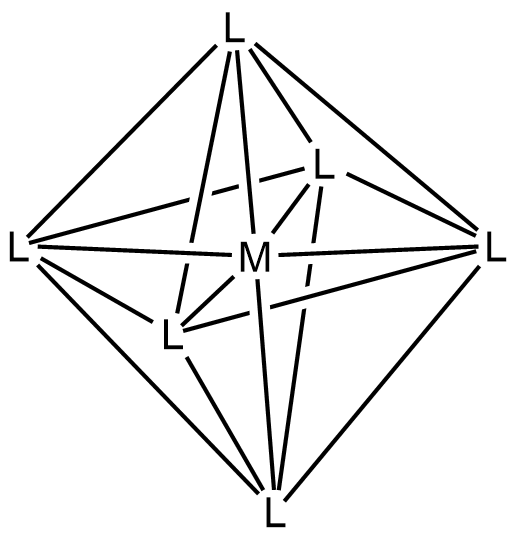
\includegraphics[width=0.30\linewidth]{figures/octahedral.png}}
\caption[Common structures of CNs]{Common structures of coordination numbers.}
\label{fig:kz}
\end{figure}